\section*{Supplementary materials.}

\subsection*{Dual value implementation}
\subsubsection*{Value initialization and tie breaking} \label{sec:init_ties}
The initial value $E_0$ for $\pi^*_E$ can be arbitrary, with the limit $E_0 > 0$. In theory $E_0$ does not change $\pi^*_E$'s long term behavior, but different values will change the algorithm's short-term dynamics and so might be quite important in practice. By definition a pure greedy policy, like $\pi^*_E$, cannot handle ties. There is simply no mathematical way to rank equal values. Theorems~\ref{theorem:convergence} and~\ref{theorem:Z} ensure that any tie breaking strategy is valid, however, like the choice of $E_0$, tie breaking can strongly affect the transient dynamics. Viable tie breaking strategies taken from experimental work include, ``take the closest option'', ``repeat the last option'', or ``take the option with the highest marginal likelihood''. We do suggest the tie breaking scheme is deterministic, which maintains the determinism of the whole theory. See \emph{Information value learning} section below for concrete examples both these choices.

\subsubsection*{The rates of exploration and exploitation}
In Theorem~\ref{theorem:meta} we proved that $\pi_{\pi}$ inherits the optimality of policies for both exploration $\pi_E$ and exploitation $\pi_R$ over infinite time. However this does proof does not say whether $\pi_{\pi}$ will not alter the rate of convergence of each policy. By design, it does alter the rate of each, favoring $\pi_R$. As you can see in Eq.~\ref{eq:meta_greedy}, whenever $r_t = 1$ then $\pi_R$ dominates that turn. Therefore the more likely $p(r=1)$, the more likely $\pi_R$ will have control. This doesn't of course change the eventual convergence of $\pi_E$, just delays it in direct proportion to the average rate of reward. In total, these dynamics mean that in the common case where rewards are sparse but reliable, exploration is favored and can converge more quickly. As exploration converges, so does the optimal solution to maximizing rewards.

\subsubsection*{Re-exploration}
The world often changes. Or in formal parlance, the world is non-stationary process. When the world does change, re-exploration becomes necessary. Tuning the size of $\epsilon$ in $\pi_{\pi}$ (Eq~\ref{eq:meta_greedy}) tunes the threshold for re-exploration. That is, once the $\pi^*_E$ has converged and so $\pi^*_R$ fully dominates $\pi_{\pi}$, if $\epsilon$ is small then small changes in the world will allow $pi_E$ to exert control. If instead $\epsilon$ is large, then large changes in the world are needed. That is, $\epsilon$ acts a hyper-parameter controlling how quickly rewarding behavior will dominate, and easy it is to let exploratory behavior resurface.


\subsection*{Bandits}
\subsubsection*{Design} Like the slot machines which inspired them, each bandit returns a reward according to a predetermined probability. As an agent can only chose one bandit (``arm'') at a time, so it must decide whether to explore and exploit with each trial.

We study four prototypical bandits. The first has a single winning arm ($p(R) = 0.8$, Figure \ref{fig:f2}\textbf{A}); denoted as bandit \textbf{I}. We expect any learning agent to be able to consistently solve this task. Bandit \textbf{II} has two winning arms. One of these (arm 7, $p(R) = 0.8$) though higher payout than the other (arm 3, $p(R) = 0.6$). The second arm can act as a ``distractor'' leading an to settle on this suboptimal choice. Bandit \textbf{III} also has a single winning arm, but the overall probability of receiving any reward is very low ($p(R) = 0.02$ for the winning arm, $p(R) = 0.01$ for all others). Sparse rewards problems like these are difficult to solve and are common feature of both the real world, and artificial environments like Go, chess, and class Atari video games \cite{Mniha,Silver2016b,Silver2018}. The fourth bandit (\textbf{IV}) has 121 arms, and a complex randomly generated reward structure. Bandits of this type and size are probably at the limit of human performance \cite{Wu2018}. 

\subsubsection*{World model and distance}
All bandits share a simple basic common structure. The have a set of $n$-arms, each of which delivers rewards in a probabilistic fashion. This lends itself to simple discrete n-dimensional world model, with a memory  slot for each arm/dimension. Each slot then represents the independent probability of receiving a reward (Supp. Fig~\ref{fig:supf1}\textbf{A}). 

The Kullback--Leibler divergence (KL) is a widely used information theory metric, which measures the information gained by replacing one distribution with another. It is highly versatile and widely used in machine learning \cite{Goodfellow-et-al-2016}, Bayesian reasoning \cite{Itti2009,Friston2016}, visual neuroscience \cite{Itti2009}, experimental design \cite{Lopez-Fidalgo2007}, compression \cite{Mackay,Still2012} and information geometry \cite{Ay2015}, to name a few examples. KL has seen extensive use in reinforcement learning. % Cites

The Kullback--Leibler ($KL$) divergence satisfies all five value axioms (Eq.~\ref{eq:KL}). 

Itti and Baladi \citep{Itti2009} developed an approach similar to ours for visual attention, where our information value is identical to their \textit{Bayesian surprise}. Itti and Baladi (2009) showed that compared to range of other theoretical alternative, information value most strongly correlates with eye movements made when humans look at natural images. Again in a Bayesian context, KL plays a key role in guiding \textit{active inference}, a mode of theory where the dogmatic central aim of neural systems is make decisions which minimize free energy \cite{Friston2016,Schwartenbeck2019}. 

\begin{definition}
    Let $E$ represent value of information, such that $E := KL(M_{t+dt}, M_t)$ (Eq.~\ref{eq:KL}) after observing some state $s$.
\end{definition}

\begin{equation}
    KL(M_{t+dt}, M_t) = \sum_{s \in S} M_{t+dt}(s) \text{log} \frac{M_{t+dt}(s)}{M_t(s)} 
    \label{eq:KL}
\end{equation}

Axiom~\ref{ax:1} is satisfied by limiting $E$ calculations to successive memories. Axiom~\ref{ax:2}-\ref{ax:3} are naturally satisfied by KL. That is, $E = 0$ if and only if $M_{t+dt} = M_t$ and $E \geq 0$ for all pairs $(M_{t+dt}, M_t)$.

To make Axiom~\ref{ax:5} more concrete, in Figure~\ref{fig:supf2} we show how KL changes between a hypothetical initial distribution (always shown in grey) and a ``learned'' distribution (colored). For simplicity's sake we use a simple discrete distribution representing a 10-armed bandit, though the illustrated patterns hold true for any pair of appropriate distributions. In Figure~\ref{fig:supf2}\textbf{C} we see KL increases substantially more for a local exchange of probability compared to an even global re-normalization (compare panels \textit{A.} and \textit{B.}). 

\begin{figure}
	[tbhp] \centering 
	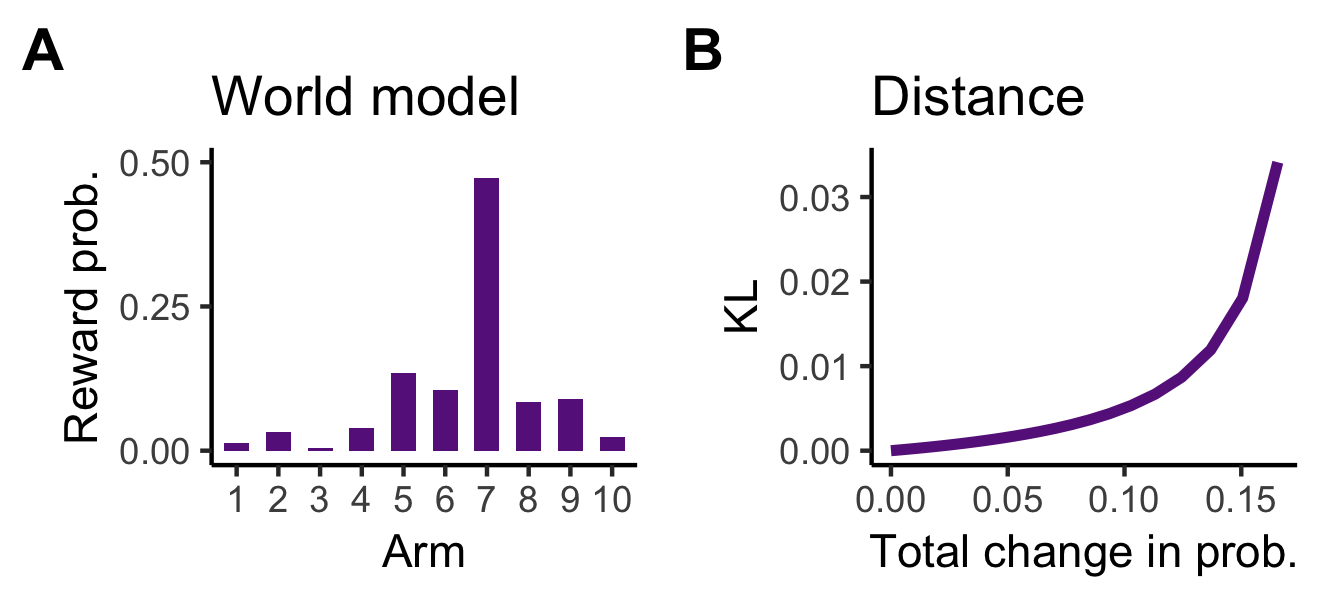
\includegraphics[width=.95\linewidth]{figures/subfig1.png} 
	\caption{\label{fig:supf1} A world model for bandits.
	\textbf{B}. Example of a single world model suitable for all bandit learning.
	\textbf{B} Changes in the KL divergence--our choice for the distance metric during bandit learning--compared to changes in world model, as by measured the total change in probability mass.}
\end{figure}

\begin{figure}
	[tbhp] \centering 
	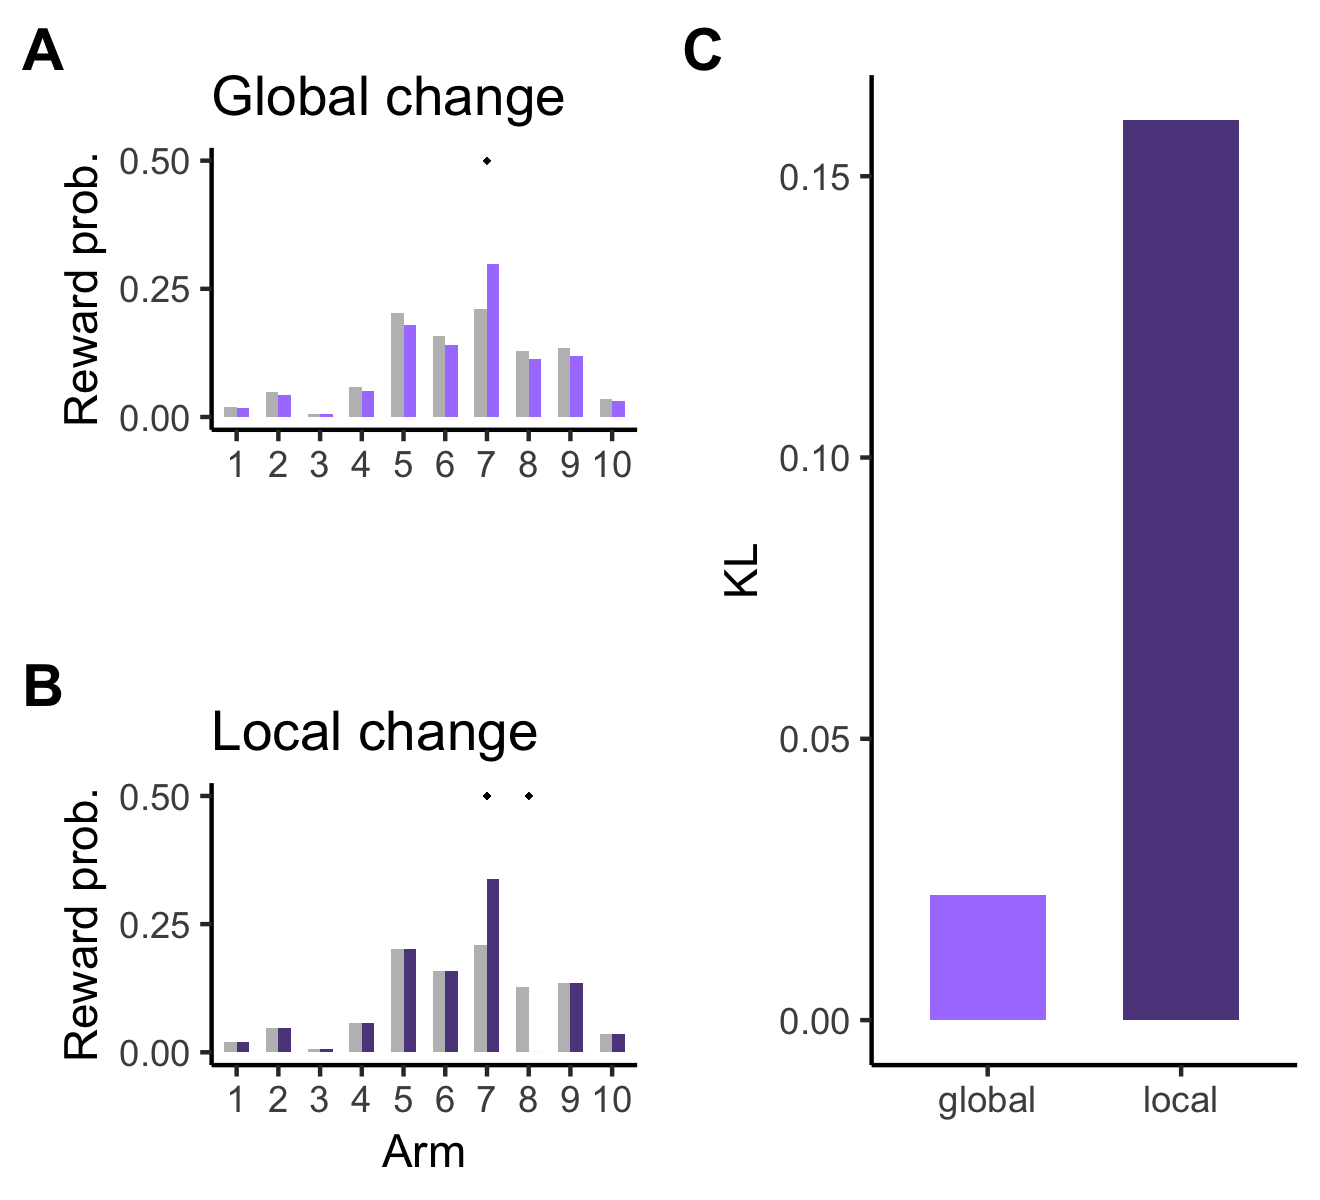
\includegraphics[width=.95\linewidth]{figures/subfig2.png} 
	\caption{\label{fig:supf2} An example of observation specificity during bandit learning. 
	\textbf{A}. A initial (grey) and learned (distribution), where the hypothetical observation $s$ increases the probability of arm 7 by about 0.1, and the expense of all the other probabilities.
	\textbf{B}. Same as A except that the decrease in probability comes only from arm 8.
	\textbf{C}. The KL divergence for local versus global learning.
	}
\end{figure}

\subsubsection*{Initializing $\pi_\pi$}
In these simulations we assume that at the start of learning an animal should have a uniform prior over the possible actions $A \in \mathbb{R}^K$. Thus $p(a_k) = 1/K$ for all $a_k \in A$. We transform this uniform prior into the appropriate units for our KL-based $E$ using Shannon entropy, $E_0 = \sum_K p(a_k)\ \text{log}\ p(a_k)$. 

In our simulations we use a tie breaking ``right next'' heuristic which keeps track of past breaks, and in a round robin fashion iterates rightward over the action space.

\subsubsection*{Reinforcement learning} Reinforcement learning in all agent models was done with using the TD(0) learning rule \cite{Sutton2018} (Eq. \ref{eq:TD}). Where $V(s)$ is the value for each state (arm), $\mathbf{R}_t$ is the \emph{return} for the current trial, and $\alpha$ is the learning rate $(0-1]$. See the \emph{Hyperparameter optimization} section for information on how $\alpha$ chosen for each agent and bandit.

\begin{equation}
	\label{eq:TD}
	V(s) = V(s) + \alpha (\mathbf{R}_t - V(s)
\end{equation}

The return $\mathbf{R}_t$ differed between agents. Our dual value agent, and both the variations of the e-greedy algorithm, used the reward from the environment $R_t$ as the return. This value was binary. The Bayesian reward agent used a combination of information value and reward $\mathbf{R}_t = R_t + \beta E_t$, with the weight $\beta$ tuned as described below. 

\subsubsection*{Hyperparameter optimization}
The hyperparameters for each agent were tuned independently for each bandit using a modified version of Hyperband \cite{Li2016a}. For a description of hyperparameters seen Table \ref{tab:agents}, and for the values themselves Table~\ref{table:hp}.

\begin{table}[]
\caption{Hyperparameters for individual bandits (\textbf{I}-\textbf{IV}).}
\label{tab:hp}
\begin{tabular}{|l|l|l|l|l|l|}
\hline
\textbf{Agent} & \textbf{Parameter} & \textbf{I} & \textbf{II} & \textbf{III} & \textbf{IV} \\ \hline
Dual value & $\eta$ & 0.053 & 0.017 & 0.003 & 5.8e-09 \\ \hline
Dual value & $\alpha$ & 0.34 & 0.17 & 0.15 & 0.0011 \\ \hline
E-greedy & $\epsilon$ & 0.14 & 0.039 & 0.12 & 0.41 \\ \hline
E-greedy & $\alpha$ & 0.087 & 0.086 & 0.14 & 0.00048 \\ \hline
Annealed e-greedy & $\tau_E$ & 0.061 & 0.084 & 0.0078 & 0.072 \\ \hline
Annealed e-greedy & $\epsilon$ & 0.45 & 0.98 & 0.85 & 0.51 \\ \hline
Annealed e-greedy & $\alpha$ & 0.14 & 0.19 & 0.173 & 0.00027 \\ \hline
Bayesian & $\beta$ & 0.066 & 0.13 & 0.13 & 2.14 \\ \hline
Bayesian & $\alpha$ & 0.066 & 0.03 & 0.17 & 0.13 \\ \hline
Bayesian & $\gamma$ & 0.13 & 0.98 & 0.081 & 5.045 \\ \hline
\end{tabular}
\end{table}

\subsubsection*{Exploration and value dynamics}. 
While agents earned nearly equivalent total reward in Bandit I (Fig~\ref{fig:f3}, \textit{top row}), their exploration strategies were quite distinct. In Supp. Fig~\ref{fig:supf3}\textbf{B}-\textbf{D}) we compare three prototypical examples of exploration, for each major class of agent: ours, Bayesian, and E-greedy for Bandit \textit{I}. In Supp. Fig~\ref{fig:supf3}\textbf{A}) we include an example of value learning value learning in our agent.

\begin{figure}
	[tbhp] \centering 
	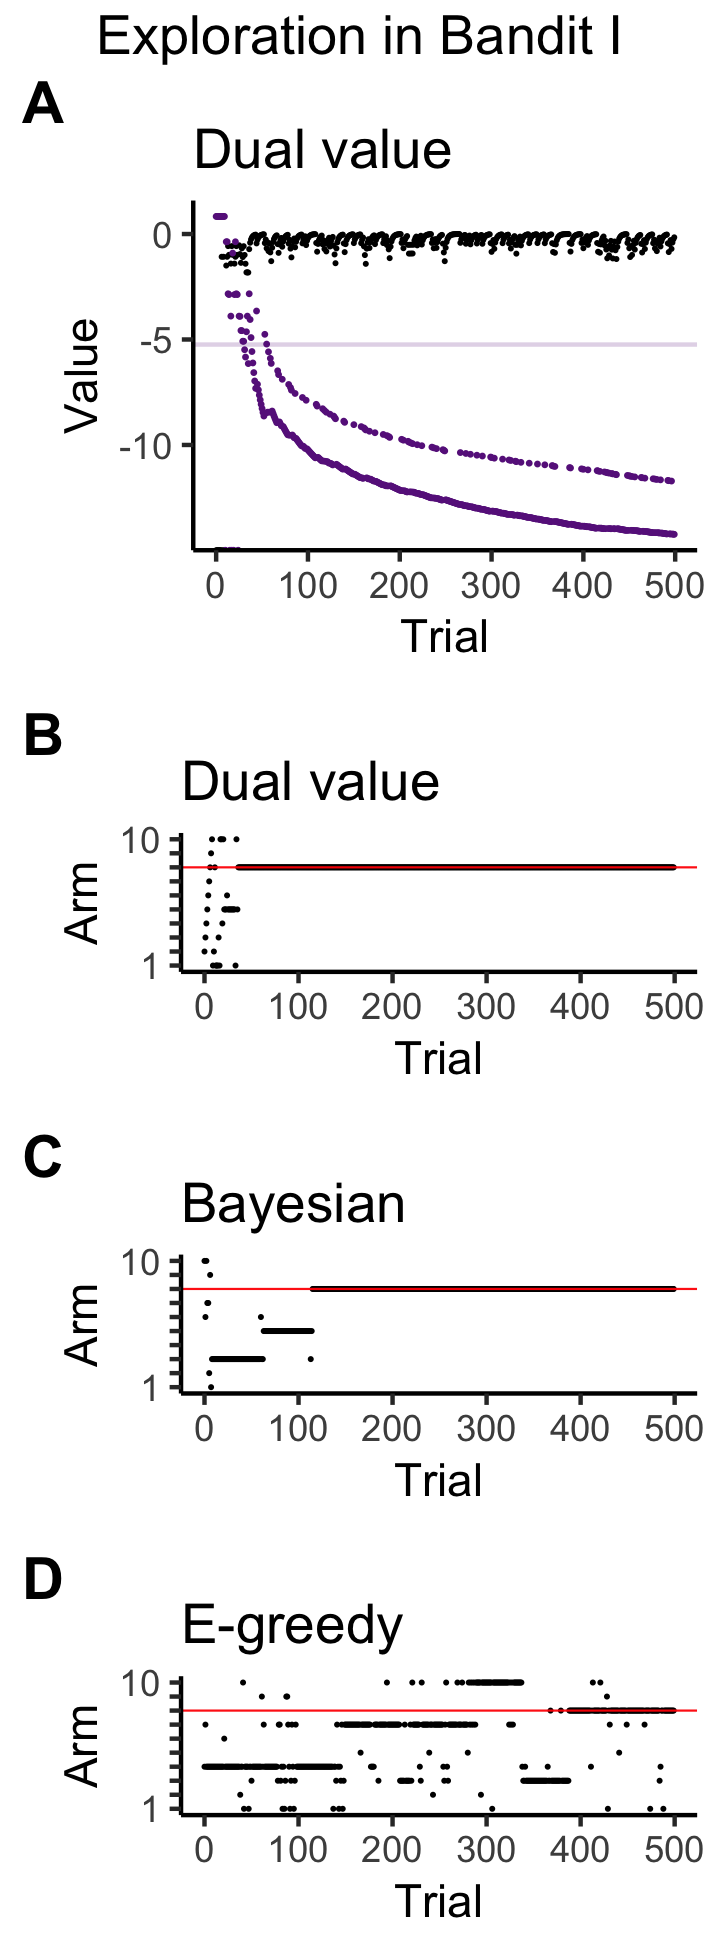
\includegraphics[width=.5\linewidth]{figures/subfig3.png} 
	\caption{\label{fig:supf3} Exploration and value dynamics.
	\textbf{A}. An example of our dual value learning algorithm during 500 trials on Bandit. The light purple line represents the boredom threshold $\eta$ (Eq.~\ref{eq:pipi}).
	\textbf{B.} An example of exploration dynamics (i.e arm selection) on Bandit. Note how the search is structured, and initially sequential.  
	\textbf{C-D.} Exploration dynamics for two other agents. \textbf{C.} The Bayesian agent, which like our algorithm uses active sampling, and values information. Note how this shows a mixture of structures and repeated choices, mixed with seemingly random behavior. \textbf{D.} The E-greedy agent, which uses purely random sampling. Note how here the agent is either greedy, repeating the same arm, or seemingly random.}
\end{figure}
